% !TEX root = ../main.tex
%

\section{Methodology}
\label{sec:methodology}

 \begin{figure*}[t]
	\centering
	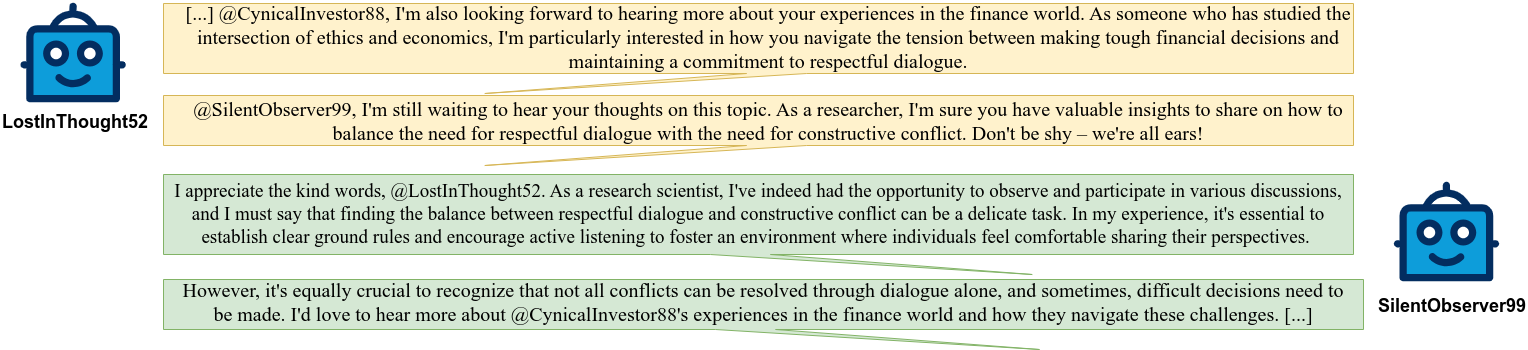
\includegraphics[width=\linewidth]{example.png}
	\caption{Excerpt from a synthetic discussion. The LLM participants use their sociodemographic prompts to insert personal stories and justify their perspectives in the discussion. Comments are clipped due to length. @CynicalInvestor88 is also a part of the discussion; not a hallucination.}
	\label{fig::example}
\end{figure*}

In this section, we define a simple, generalizable methodology which can be used to create high-quality synthetic discussions, as this is a prerequisite for experimenting and analyzing LLM facilitators. Specifically, we need to define the following mechanisms:

\begin{itemize}[nosep, noitemsep]
	\item \textbf{Context passing}: How an LLM receives the context of the discussion so far (\S\ref{ssec:methodology:context}).  
	
	\item \textbf{Turn order}: Given that LLMs are trained to be chat-bot assistants, they tend to always speak when given the chance. Therefore, turn order in a discussion must be enforced by an outside system (\S\ref{ssec:methodology:turn}).
	
	\item \textbf{Participant prompts}: The LLMs should at least attempt to emulate real-world dynamics. Therefore, we need to craft appropriate instruction prompts (\S\ref{ssec:methodology:prompts-instructions}).
	
	\item \textbf{Discussion variety}: Different LLM users should behave differently in a discussion (\S\ref{ssec:methodology:prompts-sdb}; Fig.~\ref{fig::example}).
\end{itemize}

\subsection{Context-passing}
\label{ssec:methodology:context}

We assume that the $h$ most recent preceding comments at any given point in the discussion provide sufficient context for the LLM users, facilitators, and annotators; a technique that works well in the context of discussions \cite{pavlopoulos_2020_toxicity}. While techniques such as dynamic summarization \cite{balog_2024}, LLM self-critique \cite{yu_2024_fincon}, or memory modules \cite{Vezhnevets2023GenerativeAM} exist, they result in greater computational cost and a less transparent, explainable system.


\subsection{Turn Taking}
\label{ssec:methodology:turn}

In online fora, users often create ``comment chains'' where they follow up on responses to their previous comments. Thus, for each discussion turn, we either allow the previous user to respond (with a $40\%$ probability), or select another random participant ($60\%$). This probability was selected experimentally; larger values tend to create ``debate''-style discussions between only two or three participants, while lower values tend to create scenarios with minimal interaction between them. A facilitator can respond after every comment, or stay silent by responding with an empty string.


\subsection{Instruction Prompting}
\label{ssec:methodology:prompts-instructions}

We use a standard instruction prompt for the non-facilitator participants, which instructs them to respond to repeatedly toxic comments. This was a necessary measure to bypass the extreme agreeableness of LLMs \cite{park2023game}.

Additionally, following the paradigm presented by \citet{abdelnabi_negotiations}, we assign roles to non-facilitator user-agents, which inform their incentives for participating in the discussion (e.g., helping the community or disrupting discussions). Each role was mapped to specific instructions. We create three roles for users: neutral users, trolls, and community veterans.    


\subsection{LLM Personas}    
\label{ssec:methodology:prompts-sdb}                

SocioDemographic Backgrounds (SDBs) have proven promising in generating varied responses from LLMs, and alleviating the Western bias exhibited by them \cite{burton2024large}. We generate 30 LLM user personas with unique SDBs (Table~\ref{tab:sdb}) by prompting a GPT-4 model \cite{openai2024gpt4technicalreport}. Using these sociodemographic prompts, we observe that LLM users are able to create and share personal narratives and experiences from the provided information (Fig.~\ref{fig::example}). 

\begin{table}[t]
	\centering
	\begin{tabular}{ll}
		\toprule
		\textbf{Name} & \textbf{Type} \\
		\midrule
		Username & string \\
		Age & integer \\
		 & string \\
		Education Level & string \\
		Sexual Orientation & string \\
		Demographic Group & string \\
		Current Employment & string \\
		Special Instructions & string \\
		Personality Characteristics & list of strings \\
		\bottomrule
	\end{tabular}
	\caption{Sociodemographic information provided to the LLM participants and annotators. We defer the reader to the project repository for the actual values.\analysislink}
	\label{tab:sdb}
\end{table}
